% !TeX root = ../main.tex
% Add the above to each chapter to make compiling the PDF easier in some editors.

\chapter{Reinforcement learning and DDPG}\label{chapter:introduction}

In this chapter we begin by giving a very short introduction of reinforcement learning (RL) and provide a taxonomy of the various flavors of RL. We then drill down to a specific branch in RL (model free, Q-Learning) that we plan to deploy for the portfolio optmization problem. We discuss these classes briefly before we move to explain the Deep Determinisitic Policy Gradients (DDPG) algorithm - the foundation for our solution. In the final part, we explain the different components of DDPG.

\section{Introduction to Reinforcement Learning}
Reinforcement learning (RL) is a field of machine learning that studies decision making in an environment, where an agent interacts with its surroundings to achieve a goal. The agent receives rewards based on the state it is in and the actions it takes. The aim is to maximize the cumulative reward over time by learning a function that maps optimal states to actions. The entire lifecycle is shown in Figure \ref{fig:rl_basic} \cite{wiki:reinforcement_learning}.

\begin{figure}[htpb]
  \centering
  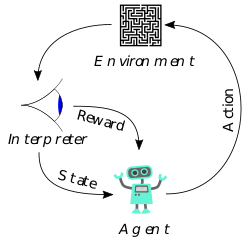
\includegraphics[width=75mm]{figures/Reinforcement_learning_diagram.png}
  \caption{Reinforcement learning} \label{fig:rl_basic}
\end{figure}

There are many flavors of RL algorithms, each targeted  at specific types of problems. A representative taxonomy of RL algorithms is provided in Figure \ref{fig:taxanomy}.

\begin{figure}[htpb]
  \centering
  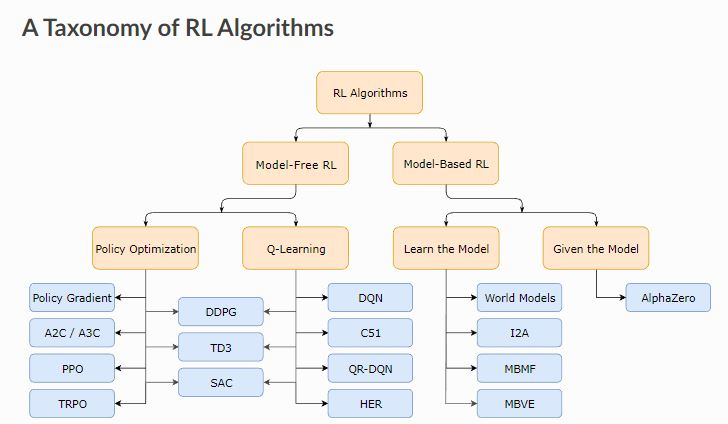
\includegraphics[width=0.8\textwidth]{figures/Taxanomy.jpg}
  \caption{Taxanomy of RL algorithms} \label{fig:taxanomy}
\end{figure}


\subsection{Model-Free vs Model-Based RL}
As can be seen in Figure \ref{fig:taxanomy}, a major classification in RL algorithms is related to the model of the environment, depending on whether or not, the model is known to the agent a priori. By model, we mean the state transition functions on taking any permissible action in the environment and also the rewards the agent obtains by taking up such an action \cite{sutton2018reinforcement}.

When the model is known to the agent, the problem is easier to solve as the agent can explicitly decide what action to take depending on the possible rewards on taking up that action. In-sample accuracy improves and training time reduces substantially when the environment can be modeled \cite{nguyen2017review}.

However in many settings, the ground truth model of the environment is  not available to the agent. 
In such cases, the agent can try to build a model based on the experience of the agent. However  such models are biased towards the training sample and quite often such agents perform terribly in real-life scenarios \cite{kaelbling1996reinforcement}.

Model-free methods on the other hand are algorithms that do not use a model of the environment, meaning they do not have a function that predicts state transitions and rewards. Instead, these methods rely solely on the experience of the agent through trial-and-error interactions with the environment. Model-free methods are easier to implement and tune compared to model-based methods, which require the agent to learn a model of the environment. Some popular model-free RL algorithms include Q-Learning, SARSA, and actor-critic networks. However, model-free methods are less sample efficient compared to model-based methods because they do not allow the agent to plan ahead. But generally they are more robust in handling real life scenarios.



\section{Q-Learning}
One of the most popular methods for solving RL problems is Q-Learning \cite{watkins1992q}, which is a model-free, off-policy algorithm. 
The basic idea behind Q-Learning is to estimate the action-value function $Q(s,a)$, also refered to as "critic", which represents the expected future reward starting from state $s$, taking action $a$ and acting optimally afterwards. The optimal action $a^*(s)$ is then computed as

\begin{equation}
a^*(s) = \arg \max_{a \in A} Q(s,a),
\end{equation}

where $A$ is the set of admissible actions.

We start off with an estimate of the $Q$ function and then iteratively update the estimate by using the Bellman optimality equation \parencite{bellman1957dynamic}


\begin{equation}
Q(s,a) \leftarrow Q(s,a) + \alpha \big[r(s,a,s') +  \max_{a' \in A} Q(s',a') - Q(s,a)\big],
\end{equation}

where $\alpha$ is the learning rate, $r(s,a,s')$ is the reward obtained after taking action $a$ in state $s$ and $s'$ is the next state.

Q-Learning has some favorable properties \cite{sutton2018reinforcement} such as:

\begin{itemize}
    \item 
    \textbf{Model-Free}: One of the key advantages of Q-Learning is that it is model free. So it is very flexible and can be applied to solve a wide range of problems.
    \item
\textbf{Off-Policy}: Q-Learning is an off-policy learner. An off-policy learner learns the value of the optimal action independently of the agent's actions. This leads to more stable results, especially when the scenarios change rapidly over time.
    \item
\textbf{Easy Implementation}: Q-Learning is a relatively simple algorithm to implement, making it a good starting point for understanding reinforcement learning.
    \item

\textbf{Good Exploration-Exploitation Trade-off}: Q-Learning balances exploration and exploitation by updating its estimates based on observed rewards. By tuning the learning rate, we can configure the exploration/exploitation trade-off at different times as we proceed into the experiment.

\end{itemize}

Q-Learning has been applied to a wide range of problems, including robot control, recommendation systems, game playing, and finance. The algorithm has been shown to be effective in many applications, but it can suffer from slow convergence and instability when applied to problems with large state spaces and sparse rewards.


One of the challenges in implementing Q-Learning is dealing with the fact that the Q-value function can have high variance. To mitigate this issue, the algorithm can be combined with function approximation techniques, such as neural networks, to approximate the value function.

\subsection{Actor - Critic Algorithm}
A variation of Q-Learning is the actor-critic algorithm \cite{konda2000actor}, which uses separate actor, $a^\phi$ and critic, $Q^\theta$ with parameters $\phi$ and $\theta$ to estimate the optimal action and the Q-value function, respectively. In other words the central underlying assumption is that $$Q(s,a) = Q^\theta(s,a)  \text{ and } a^*(s)=a^\phi(s),$$  for suitable parameterized functions $Q^\theta$ and $a^\phi$ with parameters $\theta$ and $\phi$. The actor maps states to actions, while the critic maps states and actions to a scalar value, representing the expected reward. The actor is updated based on the gradients of the Q-value function with respect to the actions, while the critic is updated using the standard Q-Learning rule. 



\section{DDPG Basics}

Deep Deterministic Policy Gradient (DDPG) is an algorithm which concurrently learns a Q-value function and an optimal action function. It uses off-policy data and the Bellman equation to learn the Q-function, and uses the Q-function to learn the policy. DDPG can only be used for environments with continuous action spaces and can be thought of as protoypical deep Q-Learning for continuous action spaces.

The DDPG approach is closely connected to Q-Learning, and is motivated by the same relation between actor $a^{\ast}$ and the critic $Q$
\begin{equation}\label{equation:Q Learning}
a^*(s) = \underset{a \in A}{\text{argmax }} Q(s,a).
\end{equation}

DDPG combines the process of learning an estimate for $Q(s,a)$ and an estimate for $a(s)$ in every update step and is tailored specifically for environments with continuous action spaces. This specialization of DDPG lies in how it calculates the maximum value of $Q(s,a)$ over all actions $a$, i.e  $\max_{a \in A} Q(s,a)$.

Finding the maximum Q-value in a scenario with a finite number of discrete actions is straightforward because we can easily evaluate the Q-values for each action and compare them, giving us the optimal action right away. However, when the action space is continuous, it's impossible to evaluate all possible actions, making the optimization problem much more complex. Using a traditional optimization algorithm to compute $\max_{a \in A} Q(s,a)$ would be computationally demanding and would have to be executed every time the agent needs to take an action, which is not practical.

Since the action space is continuous, it is assumed that the function $Q^{\theta}(s,a)$ is differentiable with respect to the action argument. This enables us to implement an efficient learning rule for the optimal action $a^\phi(s)$ that leverages this property. As a result, instead of running a costly optimization routine every time we need to calculate $\max_{a \in A} Q^\theta(s,a)$, we can approximate it as $\max_{a \in A} Q^\theta(s,a) \approx Q^\theta(s,a^\phi(s))$. 


\subsection{Algorithm}

Let us begin by stating the Bellman equation describing the optimal action-value function \cite{bellman1957dynamic} 
\begin{equation}
 Q(s,a) = \underset{s' \sim P}{{\mathbb E}}\left[r(s,a,s') +      (1-d)\max_{a'} Q(s', a')\right],   
\end{equation}


where $s' \sim P$ is shorthand for saying that the next state, $s'$, is sampled by the environment from a distribution $P(\cdot| s,a)$ and $d$ indicates whether the state $s'$ is terminal or not.

To learn an approximation of $Q(s,a)$, and $a(s)$ we use a parametrized function $Q^{\theta}(s,a)$ and $a^\phi(s)$ with parameters $\theta$ and $\phi$, and transitions $ (s,a,r,s',d)$ according to a distribution ${\mathcal D}$. We can evaluate the approximation's quality by calculating the mean-squared Bellman error (MSBE) as follows:

\begin{equation}\label{equation:Eqln}
\begin{array}{l@{}l}
L(\theta,\phi, {\mathcal D}) &{}= \underset{(s,a,r,s',d) \sim {\mathcal D}}{{\mathbb E}}\left[
    \Bigg( Q^{\theta}(s,a) - \left(r(s,a,s') +(1 - d) \max_{a'} Q^{\theta}(s',a') \right) \Bigg)^2
    \right]\\
    &{}\approx \underset{(s,a,r,s',d) \sim {\mathcal D}}{{\mathbb E}}\left[
    \Bigg( Q^{\theta}(s,a) - \left(r(s,a,s') +(1 - d) Q^{\theta}(s',a^\phi(s')) \right) \Bigg)^2
    \right]
\end{array}
\end{equation}

The Q-Learning algorithms for function approximators, including DQN and its variants as well as  DDPG, aim to minimize the MSBE loss function. These algorithms employ two key strategies and have a unique characteristic, which is specific to DDPG.

\subsubsection{Replay Buffers}

The use of an experience replay buffer is a common feature in algorithms for training deep neural networks to approximate the Q-value function, $Q(s,a)$. The replay buffer, which is a set of past experiences, must be large enough to include a diverse range of experiences, but it is important to strike a balance between having too much and too little data. Too much data may slow down the learning process, while using only the most recent data could lead to overfitting and performance issues.

It's worth noting that DDPG is an off-policy algorithm, meaning it can use experiences from outdated actions. This is possible because the Bellman equation holds for all possible transitions, regardless of how the actions were selected or what occurs after a transition. Any experiences that have been collected can be used when fitting a Q-function approximation through minimization of the mean-squared Bellman error.

\subsubsection{Target Parameters}

Several Q-Learning algorithms make use of target parameters. The term 
\begin{equation}
r(s,a,s') +(1 - d)\max_{a'} Q^{\theta}(s',a') \approx  r(s,a,s') +(1 - d) Q^{\theta}(s',a^\phi(s'))
\end{equation}
in the equation (\ref{equation:Eqln}) is called the target, because when we minimize the MSBE loss, we are trying to move the Q-value function close to this target. Q-Learning algorithms incorporate the use of target parameters to stabilize the training process. The target parameters, denoted as $\theta_{trg}$ and $\phi_{\text{trg}}$, are kept close to the actual parameters, $\theta$ and $\phi$, but with a time delay. The target parameters are used in the mean-squared Bellman error (MSBE) loss function, which is the quantity that the Q-function is trying to minimize.

To avoid instability in MSBE minimization caused by the target parameters dependence during training, the target parameters are updated periodically. In DQN algorithms, this is done by copying the actual parameters to the target every certain number of steps. In DDPG algorithms, the target parameters are obtained by weighted averaging the actual parameters and the existing target parameters with a hyperparameter $\tau$. 

\begin{equation}
\begin{array}{l@{}l}
\theta_{\text{trg}} &{}\leftarrow (1-\tau) \theta_{\text{trg}} + \tau\theta \\
\phi_{\text{trg}} &{}\leftarrow (1-\tau) \phi_{\text{trg}} + \tau\phi,

\end{array}
\end{equation}
where $\tau$ is a hyperparameter between 0 and 1 (usually close to 0). 




\subsection{Exploration vs. Exploitation}
To train the optimal allocation in DDPG, the algorithm employs an off-policy approach. To increase the exploration of previously untested actions, noise is added to the actions during training. The original DDPG paper recommends using time-correlated Ornstein-Uhlenbeck (OU) noise, but recent findings suggest that using uncorrelated, mean-zero Gaussian noise is just as effective and is simpler. It's possible to reduce the noise scale during training to improve the quality of the training data, but this is not a common practice in implementations and the noise scale is typically kept constant.
